\documentclass[main.tex]{subfiles}

\begin{document}

\section{Conclusioni}\label{sec:conclusioni}
% grafico velocità e speed up
Con questo progetto abbiamo voluto esplorare applicazioni reali della parallelizzazione nel contesto della generazione di immagini. Ci siamo divertiti nel creare mondi a nostro piacimento e testare i limiti della computazione con le GPU. \\
Partendo da un codice sequenziale che implementa un algoritmo di Ray Tracing, abbiamo applicato i paradigmi della progettazione di costrutti paralleli. Abbiamo quindi analizzato ed ottimizzato il codice sotto vari punti di vista, partendo dall'ottimizzazione del numero di thread utilizzati nei blocchi, fino ad arrivare a questioni più generiche, come la precisione dei calcoli. Abbiamo affrontato i limiti dell'algoritmo parallelizzato e proposto idee per eventuali soluzioni.
\begin{figure}[h]
    \centering
    \fbox{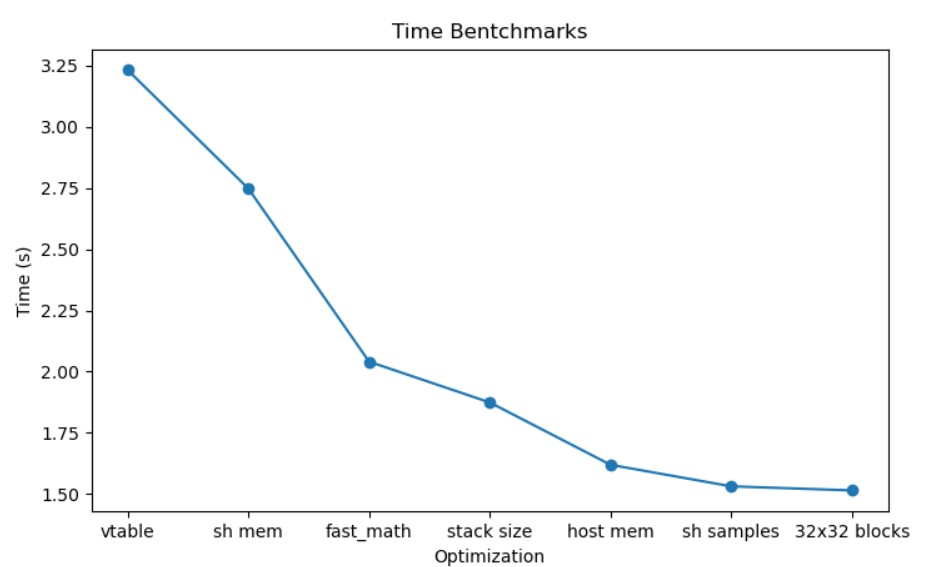
\includegraphics[width=0.9\textwidth]{figures/Ottimizzazioni_Btmrk.jpg}}
    \captionsetup{aboveskip=0pt}
    \captionof{figure}{Grafico sui Tempi di Esecuzione con le Ottimizzazioni}\vspace{-14pt}\rule{0.8\linewidth}{0.4pt}
\end{figure}\\
Nel complesso, siamo partiti da un codice sequenziale che genera l'immagine in quasi 30min e siamo riusciti ad ottenere un codice parallelo che esegue gli stessi calcoli in poco più di 1min. A seguito di analisi e varie ottimizzazioni siamo riuciti a diminuire in maggior modo il tempo di esecuzione, portandolo a 1.5s. Calcoliamo gli \textit{Speed-up}:
\begin{enumerate}
    \item  Dal codice sequenziale a quello parallelo:
\[
\text{\textit{Speed-up}} = \frac{T_{seriale}}{T_{parallelo}} = \frac{29min\ 29s}{1m\ 11s} = 24.9
\]
    \item Dal codice sequenziale a quello ottimizzato:
\[
\text{\textit{Speed-up}}_{ott} = \frac{T_{seriale}}{T_{parallelo_ott}} = \frac{29min\ 29s}{1.5s} = 1179.3
\]
\end{enumerate}

% immagine del tramonto


\end{document}